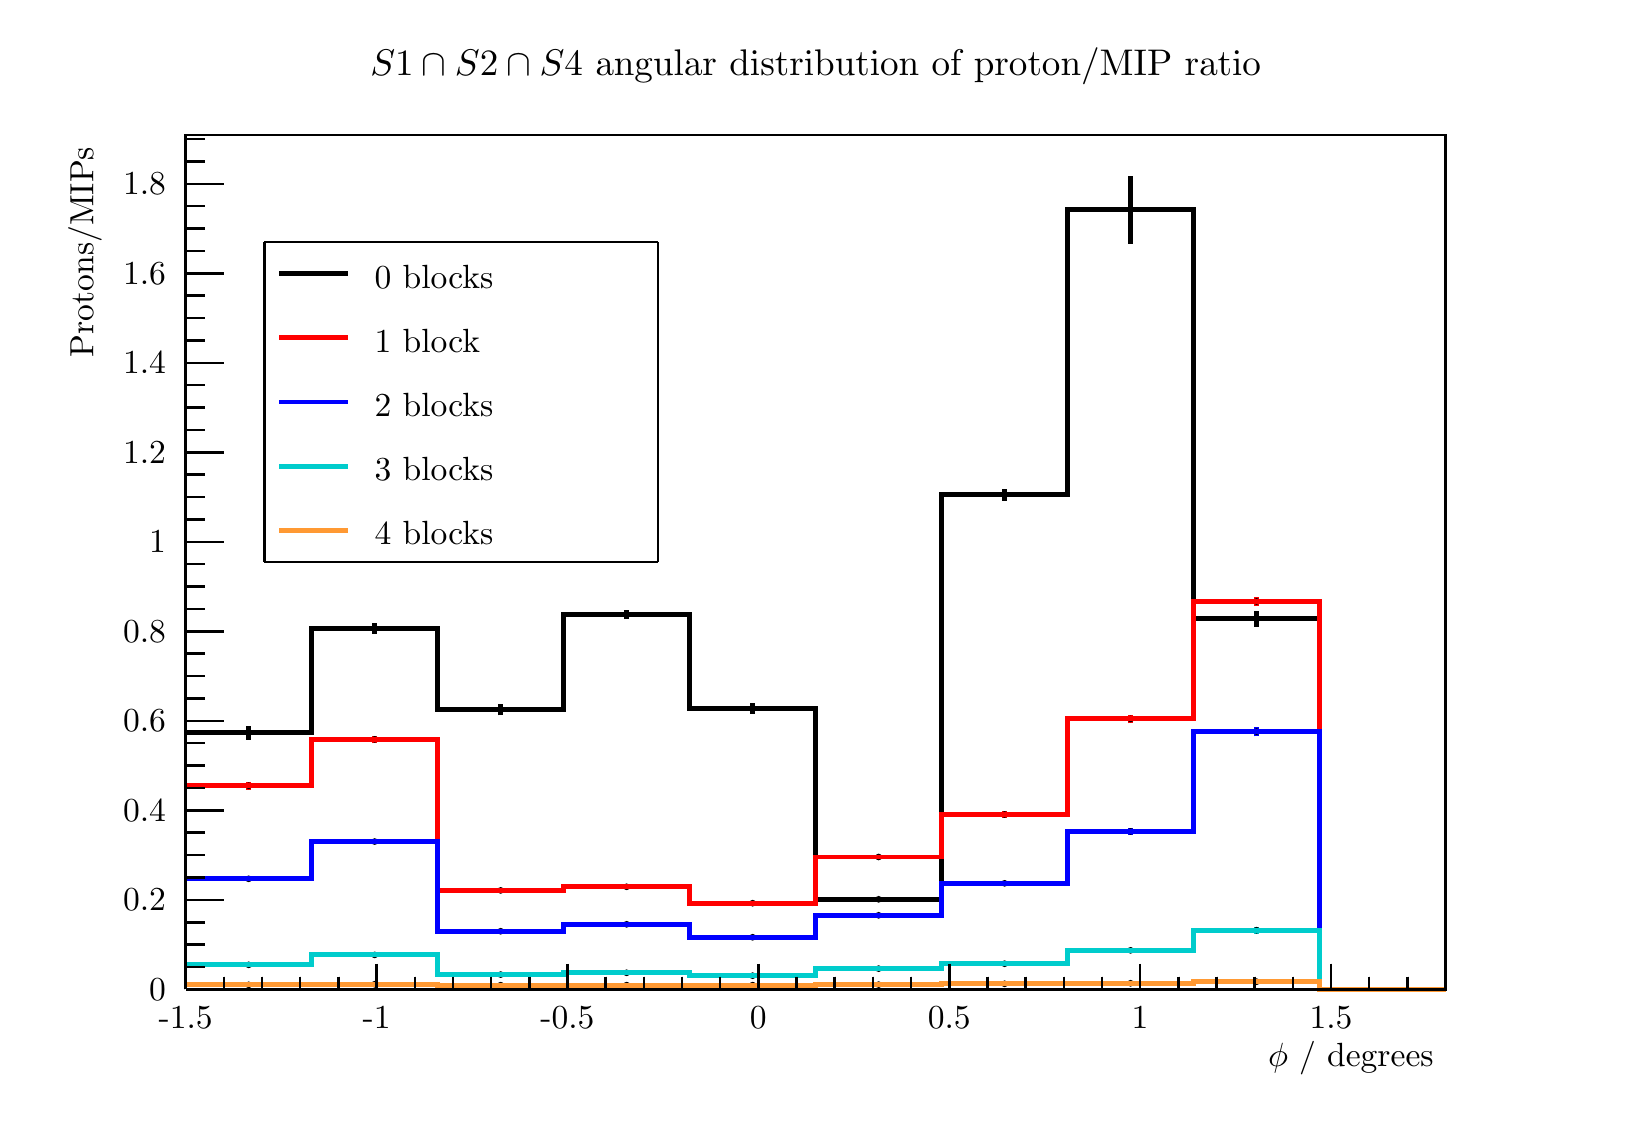
\begin{tikzpicture}
\pgfdeclareplotmark{cross} {
\pgfpathmoveto{\pgfpoint{-0.3\pgfplotmarksize}{\pgfplotmarksize}}
\pgfpathlineto{\pgfpoint{+0.3\pgfplotmarksize}{\pgfplotmarksize}}
\pgfpathlineto{\pgfpoint{+0.3\pgfplotmarksize}{0.3\pgfplotmarksize}}
\pgfpathlineto{\pgfpoint{+1\pgfplotmarksize}{0.3\pgfplotmarksize}}
\pgfpathlineto{\pgfpoint{+1\pgfplotmarksize}{-0.3\pgfplotmarksize}}
\pgfpathlineto{\pgfpoint{+0.3\pgfplotmarksize}{-0.3\pgfplotmarksize}}
\pgfpathlineto{\pgfpoint{+0.3\pgfplotmarksize}{-1.\pgfplotmarksize}}
\pgfpathlineto{\pgfpoint{-0.3\pgfplotmarksize}{-1.\pgfplotmarksize}}
\pgfpathlineto{\pgfpoint{-0.3\pgfplotmarksize}{-0.3\pgfplotmarksize}}
\pgfpathlineto{\pgfpoint{-1.\pgfplotmarksize}{-0.3\pgfplotmarksize}}
\pgfpathlineto{\pgfpoint{-1.\pgfplotmarksize}{0.3\pgfplotmarksize}}
\pgfpathlineto{\pgfpoint{-0.3\pgfplotmarksize}{0.3\pgfplotmarksize}}
\pgfpathclose
\pgfusepathqstroke
}
\pgfdeclareplotmark{cross*} {
\pgfpathmoveto{\pgfpoint{-0.3\pgfplotmarksize}{\pgfplotmarksize}}
\pgfpathlineto{\pgfpoint{+0.3\pgfplotmarksize}{\pgfplotmarksize}}
\pgfpathlineto{\pgfpoint{+0.3\pgfplotmarksize}{0.3\pgfplotmarksize}}
\pgfpathlineto{\pgfpoint{+1\pgfplotmarksize}{0.3\pgfplotmarksize}}
\pgfpathlineto{\pgfpoint{+1\pgfplotmarksize}{-0.3\pgfplotmarksize}}
\pgfpathlineto{\pgfpoint{+0.3\pgfplotmarksize}{-0.3\pgfplotmarksize}}
\pgfpathlineto{\pgfpoint{+0.3\pgfplotmarksize}{-1.\pgfplotmarksize}}
\pgfpathlineto{\pgfpoint{-0.3\pgfplotmarksize}{-1.\pgfplotmarksize}}
\pgfpathlineto{\pgfpoint{-0.3\pgfplotmarksize}{-0.3\pgfplotmarksize}}
\pgfpathlineto{\pgfpoint{-1.\pgfplotmarksize}{-0.3\pgfplotmarksize}}
\pgfpathlineto{\pgfpoint{-1.\pgfplotmarksize}{0.3\pgfplotmarksize}}
\pgfpathlineto{\pgfpoint{-0.3\pgfplotmarksize}{0.3\pgfplotmarksize}}
\pgfpathclose
\pgfusepathqfillstroke
}
\pgfdeclareplotmark{newstar} {
\pgfpathmoveto{\pgfqpoint{0pt}{\pgfplotmarksize}}
\pgfpathlineto{\pgfqpointpolar{44}{0.5\pgfplotmarksize}}
\pgfpathlineto{\pgfqpointpolar{18}{\pgfplotmarksize}}
\pgfpathlineto{\pgfqpointpolar{-20}{0.5\pgfplotmarksize}}
\pgfpathlineto{\pgfqpointpolar{-54}{\pgfplotmarksize}}
\pgfpathlineto{\pgfqpointpolar{-90}{0.5\pgfplotmarksize}}
\pgfpathlineto{\pgfqpointpolar{234}{\pgfplotmarksize}}
\pgfpathlineto{\pgfqpointpolar{198}{0.5\pgfplotmarksize}}
\pgfpathlineto{\pgfqpointpolar{162}{\pgfplotmarksize}}
\pgfpathlineto{\pgfqpointpolar{134}{0.5\pgfplotmarksize}}
\pgfpathclose
\pgfusepathqstroke
}
\pgfdeclareplotmark{newstar*} {
\pgfpathmoveto{\pgfqpoint{0pt}{\pgfplotmarksize}}
\pgfpathlineto{\pgfqpointpolar{44}{0.5\pgfplotmarksize}}
\pgfpathlineto{\pgfqpointpolar{18}{\pgfplotmarksize}}
\pgfpathlineto{\pgfqpointpolar{-20}{0.5\pgfplotmarksize}}
\pgfpathlineto{\pgfqpointpolar{-54}{\pgfplotmarksize}}
\pgfpathlineto{\pgfqpointpolar{-90}{0.5\pgfplotmarksize}}
\pgfpathlineto{\pgfqpointpolar{234}{\pgfplotmarksize}}
\pgfpathlineto{\pgfqpointpolar{198}{0.5\pgfplotmarksize}}
\pgfpathlineto{\pgfqpointpolar{162}{\pgfplotmarksize}}
\pgfpathlineto{\pgfqpointpolar{134}{0.5\pgfplotmarksize}}
\pgfpathclose
\pgfusepathqfillstroke
}
\definecolor{c}{rgb}{1,1,1};
\draw [color=c, fill=c] (0,0) rectangle (20,13.5632);
\draw [color=c, fill=c] (2,1.35632) rectangle (18,12.2069);
\definecolor{c}{rgb}{0,0,0};
\draw [c,line width=0.9] (2,1.35632) -- (2,12.2069) -- (18,12.2069) -- (18,1.35632) -- (2,1.35632);
\definecolor{c}{rgb}{1,1,1};
\draw [color=c, fill=c] (2,1.35632) rectangle (18,12.2069);
\definecolor{c}{rgb}{0,0,0};
\draw [c,line width=0.9] (2,1.35632) -- (2,12.2069) -- (18,12.2069) -- (18,1.35632) -- (2,1.35632);
\definecolor{c}{rgb}{0,0,0.6};
\draw [c,line width=0.9] (2,1.35632) -- (3.6,1.35632) -- (3.6,1.35632) -- (5.2,1.35632) -- (5.2,1.35632) -- (6.8,1.35632) -- (6.8,1.35632) -- (8.4,1.35632) -- (8.4,1.35632) -- (10,1.35632) -- (10,1.35632) -- (11.6,1.35632) -- (11.6,1.35632) --
 (13.2,1.35632) -- (13.2,1.35632) -- (14.8,1.35632) -- (14.8,1.35632) -- (16.4,1.35632) -- (16.4,1.35632) -- (18,1.35632);
\definecolor{c}{rgb}{0,0,0};
\draw [c,line width=0.9] (2,1.35632) -- (18,1.35632);
\draw [anchor= east] (18,0.488276) node[scale=1.2126, color=c, rotate=0]{$ \phi$ / degrees};
\draw [c,line width=0.9] (2,1.68184) -- (2,1.35632);
\draw [c,line width=0.9] (2.48485,1.51908) -- (2.48485,1.35632);
\draw [c,line width=0.9] (2.9697,1.51908) -- (2.9697,1.35632);
\draw [c,line width=0.9] (3.45455,1.51908) -- (3.45455,1.35632);
\draw [c,line width=0.9] (3.93939,1.51908) -- (3.93939,1.35632);
\draw [c,line width=0.9] (4.42424,1.68184) -- (4.42424,1.35632);
\draw [c,line width=0.9] (4.90909,1.51908) -- (4.90909,1.35632);
\draw [c,line width=0.9] (5.39394,1.51908) -- (5.39394,1.35632);
\draw [c,line width=0.9] (5.87879,1.51908) -- (5.87879,1.35632);
\draw [c,line width=0.9] (6.36364,1.51908) -- (6.36364,1.35632);
\draw [c,line width=0.9] (6.84848,1.68184) -- (6.84848,1.35632);
\draw [c,line width=0.9] (7.33333,1.51908) -- (7.33333,1.35632);
\draw [c,line width=0.9] (7.81818,1.51908) -- (7.81818,1.35632);
\draw [c,line width=0.9] (8.30303,1.51908) -- (8.30303,1.35632);
\draw [c,line width=0.9] (8.78788,1.51908) -- (8.78788,1.35632);
\draw [c,line width=0.9] (9.27273,1.68184) -- (9.27273,1.35632);
\draw [c,line width=0.9] (9.75758,1.51908) -- (9.75758,1.35632);
\draw [c,line width=0.9] (10.2424,1.51908) -- (10.2424,1.35632);
\draw [c,line width=0.9] (10.7273,1.51908) -- (10.7273,1.35632);
\draw [c,line width=0.9] (11.2121,1.51908) -- (11.2121,1.35632);
\draw [c,line width=0.9] (11.697,1.68184) -- (11.697,1.35632);
\draw [c,line width=0.9] (12.1818,1.51908) -- (12.1818,1.35632);
\draw [c,line width=0.9] (12.6667,1.51908) -- (12.6667,1.35632);
\draw [c,line width=0.9] (13.1515,1.51908) -- (13.1515,1.35632);
\draw [c,line width=0.9] (13.6364,1.51908) -- (13.6364,1.35632);
\draw [c,line width=0.9] (14.1212,1.68184) -- (14.1212,1.35632);
\draw [c,line width=0.9] (14.6061,1.51908) -- (14.6061,1.35632);
\draw [c,line width=0.9] (15.0909,1.51908) -- (15.0909,1.35632);
\draw [c,line width=0.9] (15.5758,1.51908) -- (15.5758,1.35632);
\draw [c,line width=0.9] (16.0606,1.51908) -- (16.0606,1.35632);
\draw [c,line width=0.9] (16.5455,1.68184) -- (16.5455,1.35632);
\draw [c,line width=0.9] (16.5455,1.68184) -- (16.5455,1.35632);
\draw [c,line width=0.9] (17.0303,1.51908) -- (17.0303,1.35632);
\draw [c,line width=0.9] (17.5152,1.51908) -- (17.5152,1.35632);
\draw [c,line width=0.9] (18,1.51908) -- (18,1.35632);
\draw [anchor=base] (2,0.854483) node[scale=1.2126, color=c, rotate=0]{-1.5};
\draw [anchor=base] (4.42424,0.854483) node[scale=1.2126, color=c, rotate=0]{-1};
\draw [anchor=base] (6.84848,0.854483) node[scale=1.2126, color=c, rotate=0]{-0.5};
\draw [anchor=base] (9.27273,0.854483) node[scale=1.2126, color=c, rotate=0]{0};
\draw [anchor=base] (11.697,0.854483) node[scale=1.2126, color=c, rotate=0]{0.5};
\draw [anchor=base] (14.1212,0.854483) node[scale=1.2126, color=c, rotate=0]{1};
\draw [anchor=base] (16.5455,0.854483) node[scale=1.2126, color=c, rotate=0]{1.5};
\draw [c,line width=0.9] (2,1.35632) -- (2,12.2069);
\draw [anchor= east] (0.72,12.2069) node[scale=1.2126, color=c, rotate=90]{ Protons/MIPs};
\draw [c,line width=0.9] (2.48,1.35632) -- (2,1.35632);
\draw [c,line width=0.9] (2.24,1.64053) -- (2,1.64053);
\draw [c,line width=0.9] (2.24,1.92473) -- (2,1.92473);
\draw [c,line width=0.9] (2.24,2.20894) -- (2,2.20894);
\draw [c,line width=0.9] (2.48,2.49314) -- (2,2.49314);
\draw [c,line width=0.9] (2.24,2.77735) -- (2,2.77735);
\draw [c,line width=0.9] (2.24,3.06155) -- (2,3.06155);
\draw [c,line width=0.9] (2.24,3.34576) -- (2,3.34576);
\draw [c,line width=0.9] (2.48,3.62996) -- (2,3.62996);
\draw [c,line width=0.9] (2.24,3.91417) -- (2,3.91417);
\draw [c,line width=0.9] (2.24,4.19837) -- (2,4.19837);
\draw [c,line width=0.9] (2.24,4.48258) -- (2,4.48258);
\draw [c,line width=0.9] (2.48,4.76678) -- (2,4.76678);
\draw [c,line width=0.9] (2.24,5.05099) -- (2,5.05099);
\draw [c,line width=0.9] (2.24,5.33519) -- (2,5.33519);
\draw [c,line width=0.9] (2.24,5.6194) -- (2,5.6194);
\draw [c,line width=0.9] (2.48,5.9036) -- (2,5.9036);
\draw [c,line width=0.9] (2.24,6.18781) -- (2,6.18781);
\draw [c,line width=0.9] (2.24,6.47201) -- (2,6.47201);
\draw [c,line width=0.9] (2.24,6.75622) -- (2,6.75622);
\draw [c,line width=0.9] (2.48,7.04042) -- (2,7.04042);
\draw [c,line width=0.9] (2.24,7.32463) -- (2,7.32463);
\draw [c,line width=0.9] (2.24,7.60883) -- (2,7.60883);
\draw [c,line width=0.9] (2.24,7.89304) -- (2,7.89304);
\draw [c,line width=0.9] (2.48,8.17724) -- (2,8.17724);
\draw [c,line width=0.9] (2.24,8.46145) -- (2,8.46145);
\draw [c,line width=0.9] (2.24,8.74565) -- (2,8.74565);
\draw [c,line width=0.9] (2.24,9.02986) -- (2,9.02986);
\draw [c,line width=0.9] (2.48,9.31406) -- (2,9.31406);
\draw [c,line width=0.9] (2.24,9.59827) -- (2,9.59827);
\draw [c,line width=0.9] (2.24,9.88247) -- (2,9.88247);
\draw [c,line width=0.9] (2.24,10.1667) -- (2,10.1667);
\draw [c,line width=0.9] (2.48,10.4509) -- (2,10.4509);
\draw [c,line width=0.9] (2.24,10.7351) -- (2,10.7351);
\draw [c,line width=0.9] (2.24,11.0193) -- (2,11.0193);
\draw [c,line width=0.9] (2.24,11.3035) -- (2,11.3035);
\draw [c,line width=0.9] (2.48,11.5877) -- (2,11.5877);
\draw [c,line width=0.9] (2.48,11.5877) -- (2,11.5877);
\draw [c,line width=0.9] (2.24,11.8719) -- (2,11.8719);
\draw [c,line width=0.9] (2.24,12.1561) -- (2,12.1561);
\draw [anchor= east] (1.9,1.35632) node[scale=1.2126, color=c, rotate=0]{0};
\draw [anchor= east] (1.9,2.49314) node[scale=1.2126, color=c, rotate=0]{0.2};
\draw [anchor= east] (1.9,3.62996) node[scale=1.2126, color=c, rotate=0]{0.4};
\draw [anchor= east] (1.9,4.76678) node[scale=1.2126, color=c, rotate=0]{0.6};
\draw [anchor= east] (1.9,5.9036) node[scale=1.2126, color=c, rotate=0]{0.8};
\draw [anchor= east] (1.9,7.04042) node[scale=1.2126, color=c, rotate=0]{1};
\draw [anchor= east] (1.9,8.17724) node[scale=1.2126, color=c, rotate=0]{1.2};
\draw [anchor= east] (1.9,9.31406) node[scale=1.2126, color=c, rotate=0]{1.4};
\draw [anchor= east] (1.9,10.4509) node[scale=1.2126, color=c, rotate=0]{1.6};
\draw [anchor= east] (1.9,11.5877) node[scale=1.2126, color=c, rotate=0]{1.8};
\draw [c,line width=1.8] (2.8,4.52786) -- (2.8,4.61649);
\draw [c,line width=1.8] (2.8,4.61649) -- (2.8,4.70512);
\foreach \P in {(2.8,4.61649)}{\draw[mark options={color=c,fill=c},mark size=2.402402pt,mark=*,mark size=1pt] plot coordinates {\P};}
\draw [c,line width=1.8] (4.4,5.87328) -- (4.4,5.94218);
\draw [c,line width=1.8] (4.4,5.94218) -- (4.4,6.01107);
\foreach \P in {(4.4,5.94218)}{\draw[mark options={color=c,fill=c},mark size=2.402402pt,mark=*,mark size=1pt] plot coordinates {\P};}
\draw [c,line width=1.8] (6,4.83657) -- (6,4.90889);
\draw [c,line width=1.8] (6,4.90889) -- (6,4.9812);
\foreach \P in {(6,4.90889)}{\draw[mark options={color=c,fill=c},mark size=2.402402pt,mark=*,mark size=1pt] plot coordinates {\P};}
\draw [c,line width=1.8] (7.6,6.05742) -- (7.6,6.11289);
\draw [c,line width=1.8] (7.6,6.11289) -- (7.6,6.16836);
\foreach \P in {(7.6,6.11289)}{\draw[mark options={color=c,fill=c},mark size=2.402402pt,mark=*,mark size=1pt] plot coordinates {\P};}
\draw [c,line width=1.8] (9.2,4.85848) -- (9.2,4.92525);
\draw [c,line width=1.8] (9.2,4.92525) -- (9.2,4.99203);
\foreach \P in {(9.2,4.92525)}{\draw[mark options={color=c,fill=c},mark size=2.402402pt,mark=*,mark size=1pt] plot coordinates {\P};}
\draw [c,line width=1.8] (10.8,2.46997) -- (10.8,2.50047);
\draw [c,line width=1.8] (10.8,2.50047) -- (10.8,2.53097);
\foreach \P in {(10.8,2.50047)}{\draw[mark options={color=c,fill=c},mark size=2.402402pt,mark=*,mark size=1pt] plot coordinates {\P};}
\draw [c,line width=1.8] (12.4,7.56489) -- (12.4,7.6379);
\draw [c,line width=1.8] (12.4,7.6379) -- (12.4,7.71091);
\foreach \P in {(12.4,7.6379)}{\draw[mark options={color=c,fill=c},mark size=2.402402pt,mark=*,mark size=1pt] plot coordinates {\P};}
\draw [c,line width=1.8] (14,10.8284) -- (14,11.2593);
\draw [c,line width=1.8] (14,11.2593) -- (14,11.6902);
\foreach \P in {(14,11.2593)}{\draw[mark options={color=c,fill=c},mark size=2.402402pt,mark=*,mark size=1pt] plot coordinates {\P};}
\draw [c,line width=1.8] (15.6,5.9618) -- (15.6,6.06082);
\draw [c,line width=1.8] (15.6,6.06082) -- (15.6,6.15984);
\foreach \P in {(15.6,6.06082)}{\draw[mark options={color=c,fill=c},mark size=2.402402pt,mark=*,mark size=1pt] plot coordinates {\P};}
\draw [c,line width=1.8] (2,4.61649) -- (3.6,4.61649) -- (3.6,5.94218) -- (5.2,5.94218) -- (5.2,4.90889) -- (6.8,4.90889) -- (6.8,6.11289) -- (8.4,6.11289) -- (8.4,4.92525) -- (10,4.92525) -- (10,2.50047) -- (11.6,2.50047) -- (11.6,7.6379) --
 (13.2,7.6379) -- (13.2,11.2593) -- (14.8,11.2593) -- (14.8,6.06082) -- (16.4,6.06082) -- (16.4,1.35632) -- (18,1.35632);
\definecolor{c}{rgb}{1,0,0};
\draw [c,line width=1.8] (2.8,3.89168) -- (2.8,3.94269);
\draw [c,line width=1.8] (2.8,3.94269) -- (2.8,3.9937);
\definecolor{c}{rgb}{0,0,0};
\foreach \P in {(2.8,3.94269)}{\draw[mark options={color=c,fill=c},mark size=2.402402pt,mark=*,mark size=1pt] plot coordinates {\P};}
\definecolor{c}{rgb}{1,0,0};
\draw [c,line width=1.8] (4.4,4.4836) -- (4.4,4.53195);
\draw [c,line width=1.8] (4.4,4.53195) -- (4.4,4.58029);
\definecolor{c}{rgb}{0,0,0};
\foreach \P in {(4.4,4.53195)}{\draw[mark options={color=c,fill=c},mark size=2.402402pt,mark=*,mark size=1pt] plot coordinates {\P};}
\definecolor{c}{rgb}{1,0,0};
\draw [c,line width=1.8] (6,2.58936) -- (6,2.61337);
\draw [c,line width=1.8] (6,2.61337) -- (6,2.63738);
\definecolor{c}{rgb}{0,0,0};
\foreach \P in {(6,2.61337)}{\draw[mark options={color=c,fill=c},mark size=2.402402pt,mark=*,mark size=1pt] plot coordinates {\P};}
\definecolor{c}{rgb}{1,0,0};
\draw [c,line width=1.8] (7.6,2.63677) -- (7.6,2.65956);
\draw [c,line width=1.8] (7.6,2.65956) -- (7.6,2.68236);
\definecolor{c}{rgb}{0,0,0};
\foreach \P in {(7.6,2.65956)}{\draw[mark options={color=c,fill=c},mark size=2.402402pt,mark=*,mark size=1pt] plot coordinates {\P};}
\definecolor{c}{rgb}{1,0,0};
\draw [c,line width=1.8] (9.2,2.43084) -- (9.2,2.45105);
\draw [c,line width=1.8] (9.2,2.45105) -- (9.2,2.47127);
\definecolor{c}{rgb}{0,0,0};
\foreach \P in {(9.2,2.45105)}{\draw[mark options={color=c,fill=c},mark size=2.402402pt,mark=*,mark size=1pt] plot coordinates {\P};}
\definecolor{c}{rgb}{1,0,0};
\draw [c,line width=1.8] (10.8,3.00958) -- (10.8,3.03783);
\draw [c,line width=1.8] (10.8,3.03783) -- (10.8,3.06608);
\definecolor{c}{rgb}{0,0,0};
\foreach \P in {(10.8,3.03783)}{\draw[mark options={color=c,fill=c},mark size=2.402402pt,mark=*,mark size=1pt] plot coordinates {\P};}
\definecolor{c}{rgb}{1,0,0};
\draw [c,line width=1.8] (12.4,3.53763) -- (12.4,3.57752);
\draw [c,line width=1.8] (12.4,3.57752) -- (12.4,3.61741);
\definecolor{c}{rgb}{0,0,0};
\foreach \P in {(12.4,3.57752)}{\draw[mark options={color=c,fill=c},mark size=2.402402pt,mark=*,mark size=1pt] plot coordinates {\P};}
\definecolor{c}{rgb}{1,0,0};
\draw [c,line width=1.8] (14,4.73628) -- (14,4.79116);
\draw [c,line width=1.8] (14,4.79116) -- (14,4.84604);
\definecolor{c}{rgb}{0,0,0};
\foreach \P in {(14,4.79116)}{\draw[mark options={color=c,fill=c},mark size=2.402402pt,mark=*,mark size=1pt] plot coordinates {\P};}
\definecolor{c}{rgb}{1,0,0};
\draw [c,line width=1.8] (15.6,6.2245) -- (15.6,6.28324);
\draw [c,line width=1.8] (15.6,6.28324) -- (15.6,6.34199);
\definecolor{c}{rgb}{0,0,0};
\foreach \P in {(15.6,6.28324)}{\draw[mark options={color=c,fill=c},mark size=2.402402pt,mark=*,mark size=1pt] plot coordinates {\P};}
\definecolor{c}{rgb}{1,0,0};
\draw [c,line width=1.8] (2,3.94269) -- (3.6,3.94269) -- (3.6,4.53195) -- (5.2,4.53195) -- (5.2,2.61337) -- (6.8,2.61337) -- (6.8,2.65956) -- (8.4,2.65956) -- (8.4,2.45105) -- (10,2.45105) -- (10,3.03783) -- (11.6,3.03783) -- (11.6,3.57752) --
 (13.2,3.57752) -- (13.2,4.79116) -- (14.8,4.79116) -- (14.8,6.28324) -- (16.4,6.28324) -- (16.4,1.35632) -- (18,1.35632);
\definecolor{c}{rgb}{0,0,1};
\draw [c,line width=1.8] (2.8,2.7273) -- (2.8,2.76072);
\draw [c,line width=1.8] (2.8,2.76072) -- (2.8,2.79413);
\definecolor{c}{rgb}{0,0,0};
\foreach \P in {(2.8,2.76072)}{\draw[mark options={color=c,fill=c},mark size=2.402402pt,mark=*,mark size=1pt] plot coordinates {\P};}
\definecolor{c}{rgb}{0,0,1};
\draw [c,line width=1.8] (4.4,3.1989) -- (4.4,3.23402);
\draw [c,line width=1.8] (4.4,3.23402) -- (4.4,3.26914);
\definecolor{c}{rgb}{0,0,0};
\foreach \P in {(4.4,3.23402)}{\draw[mark options={color=c,fill=c},mark size=2.402402pt,mark=*,mark size=1pt] plot coordinates {\P};}
\definecolor{c}{rgb}{0,0,1};
\draw [c,line width=1.8] (6,2.07976) -- (6,2.09479);
\draw [c,line width=1.8] (6,2.09479) -- (6,2.10982);
\definecolor{c}{rgb}{0,0,0};
\foreach \P in {(6,2.09479)}{\draw[mark options={color=c,fill=c},mark size=2.402402pt,mark=*,mark size=1pt] plot coordinates {\P};}
\definecolor{c}{rgb}{0,0,1};
\draw [c,line width=1.8] (7.6,2.16804) -- (7.6,2.18299);
\draw [c,line width=1.8] (7.6,2.18299) -- (7.6,2.19795);
\definecolor{c}{rgb}{0,0,0};
\foreach \P in {(7.6,2.18299)}{\draw[mark options={color=c,fill=c},mark size=2.402402pt,mark=*,mark size=1pt] plot coordinates {\P};}
\definecolor{c}{rgb}{0,0,1};
\draw [c,line width=1.8] (9.2,2.00565) -- (9.2,2.01848);
\draw [c,line width=1.8] (9.2,2.01848) -- (9.2,2.03132);
\definecolor{c}{rgb}{0,0,0};
\foreach \P in {(9.2,2.01848)}{\draw[mark options={color=c,fill=c},mark size=2.402402pt,mark=*,mark size=1pt] plot coordinates {\P};}
\definecolor{c}{rgb}{0,0,1};
\draw [c,line width=1.8] (10.8,2.27928) -- (10.8,2.29724);
\draw [c,line width=1.8] (10.8,2.29724) -- (10.8,2.3152);
\definecolor{c}{rgb}{0,0,0};
\foreach \P in {(10.8,2.29724)}{\draw[mark options={color=c,fill=c},mark size=2.402402pt,mark=*,mark size=1pt] plot coordinates {\P};}
\definecolor{c}{rgb}{0,0,1};
\draw [c,line width=1.8] (12.4,2.67601) -- (12.4,2.70318);
\draw [c,line width=1.8] (12.4,2.70318) -- (12.4,2.73035);
\definecolor{c}{rgb}{0,0,0};
\foreach \P in {(12.4,2.70318)}{\draw[mark options={color=c,fill=c},mark size=2.402402pt,mark=*,mark size=1pt] plot coordinates {\P};}
\definecolor{c}{rgb}{0,0,1};
\draw [c,line width=1.8] (14,3.32317) -- (14,3.3629);
\draw [c,line width=1.8] (14,3.3629) -- (14,3.40264);
\definecolor{c}{rgb}{0,0,0};
\foreach \P in {(14,3.3629)}{\draw[mark options={color=c,fill=c},mark size=2.402402pt,mark=*,mark size=1pt] plot coordinates {\P};}
\definecolor{c}{rgb}{0,0,1};
\draw [c,line width=1.8] (15.6,4.56937) -- (15.6,4.63071);
\draw [c,line width=1.8] (15.6,4.63071) -- (15.6,4.69205);
\definecolor{c}{rgb}{0,0,0};
\foreach \P in {(15.6,4.63071)}{\draw[mark options={color=c,fill=c},mark size=2.402402pt,mark=*,mark size=1pt] plot coordinates {\P};}
\definecolor{c}{rgb}{0,0,1};
\draw [c,line width=1.8] (2,2.76072) -- (3.6,2.76072) -- (3.6,3.23402) -- (5.2,3.23402) -- (5.2,2.09479) -- (6.8,2.09479) -- (6.8,2.18299) -- (8.4,2.18299) -- (8.4,2.01848) -- (10,2.01848) -- (10,2.29724) -- (11.6,2.29724) -- (11.6,2.70318) --
 (13.2,2.70318) -- (13.2,3.3629) -- (14.8,3.3629) -- (14.8,4.63071) -- (16.4,4.63071) -- (16.4,1.35632) -- (18,1.35632);
\definecolor{c}{rgb}{0,0.8,0.8};
\draw [c,line width=1.8] (2.8,1.65005) -- (2.8,1.66824);
\draw [c,line width=1.8] (2.8,1.66824) -- (2.8,1.68643);
\definecolor{c}{rgb}{0,0,0};
\foreach \P in {(2.8,1.66824)}{\draw[mark options={color=c,fill=c},mark size=2.402402pt,mark=*,mark size=1pt] plot coordinates {\P};}
\definecolor{c}{rgb}{0,0.8,0.8};
\draw [c,line width=1.8] (4.4,1.77412) -- (4.4,1.7946);
\draw [c,line width=1.8] (4.4,1.7946) -- (4.4,1.81507);
\definecolor{c}{rgb}{0,0,0};
\foreach \P in {(4.4,1.7946)}{\draw[mark options={color=c,fill=c},mark size=2.402402pt,mark=*,mark size=1pt] plot coordinates {\P};}
\definecolor{c}{rgb}{0,0.8,0.8};
\draw [c,line width=1.8] (6,1.53592) -- (6,1.54425);
\draw [c,line width=1.8] (6,1.54425) -- (6,1.55258);
\definecolor{c}{rgb}{0,0,0};
\foreach \P in {(6,1.54425)}{\draw[mark options={color=c,fill=c},mark size=2.402402pt,mark=*,mark size=1pt] plot coordinates {\P};}
\definecolor{c}{rgb}{0,0.8,0.8};
\draw [c,line width=1.8] (7.6,1.55892) -- (7.6,1.56732);
\draw [c,line width=1.8] (7.6,1.56732) -- (7.6,1.57572);
\definecolor{c}{rgb}{0,0,0};
\foreach \P in {(7.6,1.56732)}{\draw[mark options={color=c,fill=c},mark size=2.402402pt,mark=*,mark size=1pt] plot coordinates {\P};}
\definecolor{c}{rgb}{0,0.8,0.8};
\draw [c,line width=1.8] (9.2,1.52312) -- (9.2,1.53036);
\draw [c,line width=1.8] (9.2,1.53036) -- (9.2,1.5376);
\definecolor{c}{rgb}{0,0,0};
\foreach \P in {(9.2,1.53036)}{\draw[mark options={color=c,fill=c},mark size=2.402402pt,mark=*,mark size=1pt] plot coordinates {\P};}
\definecolor{c}{rgb}{0,0.8,0.8};
\draw [c,line width=1.8] (10.8,1.60929) -- (10.8,1.61987);
\draw [c,line width=1.8] (10.8,1.61987) -- (10.8,1.63045);
\definecolor{c}{rgb}{0,0,0};
\foreach \P in {(10.8,1.61987)}{\draw[mark options={color=c,fill=c},mark size=2.402402pt,mark=*,mark size=1pt] plot coordinates {\P};}
\definecolor{c}{rgb}{0,0.8,0.8};
\draw [c,line width=1.8] (12.4,1.66665) -- (12.4,1.68218);
\draw [c,line width=1.8] (12.4,1.68218) -- (12.4,1.69771);
\definecolor{c}{rgb}{0,0,0};
\foreach \P in {(12.4,1.68218)}{\draw[mark options={color=c,fill=c},mark size=2.402402pt,mark=*,mark size=1pt] plot coordinates {\P};}
\definecolor{c}{rgb}{0,0.8,0.8};
\draw [c,line width=1.8] (14,1.82799) -- (14,1.85229);
\draw [c,line width=1.8] (14,1.85229) -- (14,1.8766);
\definecolor{c}{rgb}{0,0,0};
\foreach \P in {(14,1.85229)}{\draw[mark options={color=c,fill=c},mark size=2.402402pt,mark=*,mark size=1pt] plot coordinates {\P};}
\definecolor{c}{rgb}{0,0.8,0.8};
\draw [c,line width=1.8] (15.6,2.06381) -- (15.6,2.10801);
\draw [c,line width=1.8] (15.6,2.10801) -- (15.6,2.15221);
\definecolor{c}{rgb}{0,0,0};
\foreach \P in {(15.6,2.10801)}{\draw[mark options={color=c,fill=c},mark size=2.402402pt,mark=*,mark size=1pt] plot coordinates {\P};}
\definecolor{c}{rgb}{0,0.8,0.8};
\draw [c,line width=1.8] (2,1.66824) -- (3.6,1.66824) -- (3.6,1.7946) -- (5.2,1.7946) -- (5.2,1.54425) -- (6.8,1.54425) -- (6.8,1.56732) -- (8.4,1.56732) -- (8.4,1.53036) -- (10,1.53036) -- (10,1.61987) -- (11.6,1.61987) -- (11.6,1.68218) --
 (13.2,1.68218) -- (13.2,1.85229) -- (14.8,1.85229) -- (14.8,2.10801) -- (16.4,2.10801) -- (16.4,1.35632) -- (18,1.35632);
\definecolor{c}{rgb}{1,0.6,0.2};
\draw [c,line width=1.8] (2.8,1.41274) -- (2.8,1.41433);
\draw [c,line width=1.8] (2.8,1.41433) -- (2.8,1.41592);
\definecolor{c}{rgb}{0,0,0};
\foreach \P in {(2.8,1.41433)}{\draw[mark options={color=c,fill=c},mark size=2.402402pt,mark=*,mark size=1pt] plot coordinates {\P};}
\definecolor{c}{rgb}{1,0.6,0.2};
\draw [c,line width=1.8] (4.4,1.42029) -- (4.4,1.42182);
\draw [c,line width=1.8] (4.4,1.42182) -- (4.4,1.42336);
\definecolor{c}{rgb}{0,0,0};
\foreach \P in {(4.4,1.42182)}{\draw[mark options={color=c,fill=c},mark size=2.402402pt,mark=*,mark size=1pt] plot coordinates {\P};}
\definecolor{c}{rgb}{1,0.6,0.2};
\draw [c,line width=1.8] (6,1.40859) -- (6,1.40946);
\draw [c,line width=1.8] (6,1.40946) -- (6,1.41033);
\definecolor{c}{rgb}{0,0,0};
\foreach \P in {(6,1.40946)}{\draw[mark options={color=c,fill=c},mark size=2.402402pt,mark=*,mark size=1pt] plot coordinates {\P};}
\definecolor{c}{rgb}{1,0.6,0.2};
\draw [c,line width=1.8] (7.6,1.40953) -- (7.6,1.41037);
\draw [c,line width=1.8] (7.6,1.41037) -- (7.6,1.41122);
\definecolor{c}{rgb}{0,0,0};
\foreach \P in {(7.6,1.41037)}{\draw[mark options={color=c,fill=c},mark size=2.402402pt,mark=*,mark size=1pt] plot coordinates {\P};}
\definecolor{c}{rgb}{1,0.6,0.2};
\draw [c,line width=1.8] (9.2,1.40941) -- (9.2,1.41022);
\draw [c,line width=1.8] (9.2,1.41022) -- (9.2,1.41102);
\definecolor{c}{rgb}{0,0,0};
\foreach \P in {(9.2,1.41022)}{\draw[mark options={color=c,fill=c},mark size=2.402402pt,mark=*,mark size=1pt] plot coordinates {\P};}
\definecolor{c}{rgb}{1,0.6,0.2};
\draw [c,line width=1.8] (10.8,1.41566) -- (10.8,1.41668);
\draw [c,line width=1.8] (10.8,1.41668) -- (10.8,1.4177);
\definecolor{c}{rgb}{0,0,0};
\foreach \P in {(10.8,1.41668)}{\draw[mark options={color=c,fill=c},mark size=2.402402pt,mark=*,mark size=1pt] plot coordinates {\P};}
\definecolor{c}{rgb}{1,0.6,0.2};
\draw [c,line width=1.8] (12.4,1.4259) -- (12.4,1.42736);
\draw [c,line width=1.8] (12.4,1.42736) -- (12.4,1.42883);
\definecolor{c}{rgb}{0,0,0};
\foreach \P in {(12.4,1.42736)}{\draw[mark options={color=c,fill=c},mark size=2.402402pt,mark=*,mark size=1pt] plot coordinates {\P};}
\definecolor{c}{rgb}{1,0.6,0.2};
\draw [c,line width=1.8] (14,1.43199) -- (14,1.43389);
\draw [c,line width=1.8] (14,1.43389) -- (14,1.43578);
\definecolor{c}{rgb}{0,0,0};
\foreach \P in {(14,1.43389)}{\draw[mark options={color=c,fill=c},mark size=2.402402pt,mark=*,mark size=1pt] plot coordinates {\P};}
\definecolor{c}{rgb}{1,0.6,0.2};
\draw [c,line width=1.8] (15.6,1.45109) -- (15.6,1.45416);
\draw [c,line width=1.8] (15.6,1.45416) -- (15.6,1.45724);
\definecolor{c}{rgb}{0,0,0};
\foreach \P in {(15.6,1.45416)}{\draw[mark options={color=c,fill=c},mark size=2.402402pt,mark=*,mark size=1pt] plot coordinates {\P};}
\definecolor{c}{rgb}{1,0.6,0.2};
\draw [c,line width=1.8] (2,1.41433) -- (3.6,1.41433) -- (3.6,1.42182) -- (5.2,1.42182) -- (5.2,1.40946) -- (6.8,1.40946) -- (6.8,1.41037) -- (8.4,1.41037) -- (8.4,1.41022) -- (10,1.41022) -- (10,1.41668) -- (11.6,1.41668) -- (11.6,1.42736) --
 (13.2,1.42736) -- (13.2,1.43389) -- (14.8,1.43389) -- (14.8,1.45416) -- (16.4,1.45416) -- (16.4,1.35632) -- (18,1.35632);
\definecolor{c}{rgb}{0,0,0};
\draw [c,line width=0.9] (2,1.35632) -- (18,1.35632);
\draw [c,line width=0.9] (2,1.68184) -- (2,1.35632);
\draw [c,line width=0.9] (2.48485,1.51908) -- (2.48485,1.35632);
\draw [c,line width=0.9] (2.9697,1.51908) -- (2.9697,1.35632);
\draw [c,line width=0.9] (3.45455,1.51908) -- (3.45455,1.35632);
\draw [c,line width=0.9] (3.93939,1.51908) -- (3.93939,1.35632);
\draw [c,line width=0.9] (4.42424,1.68184) -- (4.42424,1.35632);
\draw [c,line width=0.9] (4.90909,1.51908) -- (4.90909,1.35632);
\draw [c,line width=0.9] (5.39394,1.51908) -- (5.39394,1.35632);
\draw [c,line width=0.9] (5.87879,1.51908) -- (5.87879,1.35632);
\draw [c,line width=0.9] (6.36364,1.51908) -- (6.36364,1.35632);
\draw [c,line width=0.9] (6.84848,1.68184) -- (6.84848,1.35632);
\draw [c,line width=0.9] (7.33333,1.51908) -- (7.33333,1.35632);
\draw [c,line width=0.9] (7.81818,1.51908) -- (7.81818,1.35632);
\draw [c,line width=0.9] (8.30303,1.51908) -- (8.30303,1.35632);
\draw [c,line width=0.9] (8.78788,1.51908) -- (8.78788,1.35632);
\draw [c,line width=0.9] (9.27273,1.68184) -- (9.27273,1.35632);
\draw [c,line width=0.9] (9.75758,1.51908) -- (9.75758,1.35632);
\draw [c,line width=0.9] (10.2424,1.51908) -- (10.2424,1.35632);
\draw [c,line width=0.9] (10.7273,1.51908) -- (10.7273,1.35632);
\draw [c,line width=0.9] (11.2121,1.51908) -- (11.2121,1.35632);
\draw [c,line width=0.9] (11.697,1.68184) -- (11.697,1.35632);
\draw [c,line width=0.9] (12.1818,1.51908) -- (12.1818,1.35632);
\draw [c,line width=0.9] (12.6667,1.51908) -- (12.6667,1.35632);
\draw [c,line width=0.9] (13.1515,1.51908) -- (13.1515,1.35632);
\draw [c,line width=0.9] (13.6364,1.51908) -- (13.6364,1.35632);
\draw [c,line width=0.9] (14.1212,1.68184) -- (14.1212,1.35632);
\draw [c,line width=0.9] (14.6061,1.51908) -- (14.6061,1.35632);
\draw [c,line width=0.9] (15.0909,1.51908) -- (15.0909,1.35632);
\draw [c,line width=0.9] (15.5758,1.51908) -- (15.5758,1.35632);
\draw [c,line width=0.9] (16.0606,1.51908) -- (16.0606,1.35632);
\draw [c,line width=0.9] (16.5455,1.68184) -- (16.5455,1.35632);
\draw [c,line width=0.9] (16.5455,1.68184) -- (16.5455,1.35632);
\draw [c,line width=0.9] (17.0303,1.51908) -- (17.0303,1.35632);
\draw [c,line width=0.9] (17.5152,1.51908) -- (17.5152,1.35632);
\draw [c,line width=0.9] (18,1.51908) -- (18,1.35632);
\draw [c,line width=0.9] (2,1.35632) -- (2,12.2069);
\draw [c,line width=0.9] (2.48,1.35632) -- (2,1.35632);
\draw [c,line width=0.9] (2.24,1.64053) -- (2,1.64053);
\draw [c,line width=0.9] (2.24,1.92473) -- (2,1.92473);
\draw [c,line width=0.9] (2.24,2.20894) -- (2,2.20894);
\draw [c,line width=0.9] (2.48,2.49314) -- (2,2.49314);
\draw [c,line width=0.9] (2.24,2.77735) -- (2,2.77735);
\draw [c,line width=0.9] (2.24,3.06155) -- (2,3.06155);
\draw [c,line width=0.9] (2.24,3.34576) -- (2,3.34576);
\draw [c,line width=0.9] (2.48,3.62996) -- (2,3.62996);
\draw [c,line width=0.9] (2.24,3.91417) -- (2,3.91417);
\draw [c,line width=0.9] (2.24,4.19837) -- (2,4.19837);
\draw [c,line width=0.9] (2.24,4.48258) -- (2,4.48258);
\draw [c,line width=0.9] (2.48,4.76678) -- (2,4.76678);
\draw [c,line width=0.9] (2.24,5.05099) -- (2,5.05099);
\draw [c,line width=0.9] (2.24,5.33519) -- (2,5.33519);
\draw [c,line width=0.9] (2.24,5.6194) -- (2,5.6194);
\draw [c,line width=0.9] (2.48,5.9036) -- (2,5.9036);
\draw [c,line width=0.9] (2.24,6.18781) -- (2,6.18781);
\draw [c,line width=0.9] (2.24,6.47201) -- (2,6.47201);
\draw [c,line width=0.9] (2.24,6.75622) -- (2,6.75622);
\draw [c,line width=0.9] (2.48,7.04042) -- (2,7.04042);
\draw [c,line width=0.9] (2.24,7.32463) -- (2,7.32463);
\draw [c,line width=0.9] (2.24,7.60883) -- (2,7.60883);
\draw [c,line width=0.9] (2.24,7.89304) -- (2,7.89304);
\draw [c,line width=0.9] (2.48,8.17724) -- (2,8.17724);
\draw [c,line width=0.9] (2.24,8.46145) -- (2,8.46145);
\draw [c,line width=0.9] (2.24,8.74565) -- (2,8.74565);
\draw [c,line width=0.9] (2.24,9.02986) -- (2,9.02986);
\draw [c,line width=0.9] (2.48,9.31406) -- (2,9.31406);
\draw [c,line width=0.9] (2.24,9.59827) -- (2,9.59827);
\draw [c,line width=0.9] (2.24,9.88247) -- (2,9.88247);
\draw [c,line width=0.9] (2.24,10.1667) -- (2,10.1667);
\draw [c,line width=0.9] (2.48,10.4509) -- (2,10.4509);
\draw [c,line width=0.9] (2.24,10.7351) -- (2,10.7351);
\draw [c,line width=0.9] (2.24,11.0193) -- (2,11.0193);
\draw [c,line width=0.9] (2.24,11.3035) -- (2,11.3035);
\draw [c,line width=0.9] (2.48,11.5877) -- (2,11.5877);
\draw [c,line width=0.9] (2.48,11.5877) -- (2,11.5877);
\draw [c,line width=0.9] (2.24,11.8719) -- (2,11.8719);
\draw [c,line width=0.9] (2.24,12.1561) -- (2,12.1561);
\draw (10,13.0816) node[scale=1.34024, color=c, rotate=0]{$S1 \cap S2 \cap S4$ angular distribution of proton/MIP ratio};
\definecolor{c}{rgb}{1,1,1};
\draw [color=c, fill=c] (3,6.78161) rectangle (8,10.8506);
\definecolor{c}{rgb}{0,0,0};
\draw [c,line width=0.9] (3,6.78161) -- (8,6.78161);
\draw [c,line width=0.9] (8,6.78161) -- (8,10.8506);
\draw [c,line width=0.9] (8,10.8506) -- (3,10.8506);
\draw [c,line width=0.9] (3,10.8506) -- (3,6.78161);
\draw [anchor=base west] (4.25,10.2606) node[scale=1.2126, color=c, rotate=0]{0 blocks};
\draw [c,line width=1.8] (3.1875,10.4437) -- (4.0625,10.4437);
\draw [anchor=base west] (4.25,9.44678) node[scale=1.2126, color=c, rotate=0]{1 block};
\definecolor{c}{rgb}{1,0,0};
\draw [c,line width=1.8] (3.1875,9.62988) -- (4.0625,9.62988);
\definecolor{c}{rgb}{0,0,0};
\draw [anchor=base west] (4.25,8.63299) node[scale=1.2126, color=c, rotate=0]{2 blocks};
\definecolor{c}{rgb}{0,0,1};
\draw [c,line width=1.8] (3.1875,8.81609) -- (4.0625,8.81609);
\definecolor{c}{rgb}{0,0,0};
\draw [anchor=base west] (4.25,7.8192) node[scale=1.2126, color=c, rotate=0]{3 blocks};
\definecolor{c}{rgb}{0,0.8,0.8};
\draw [c,line width=1.8] (3.1875,8.0023) -- (4.0625,8.0023);
\definecolor{c}{rgb}{0,0,0};
\draw [anchor=base west] (4.25,7.0054) node[scale=1.2126, color=c, rotate=0]{4 blocks};
\definecolor{c}{rgb}{1,0.6,0.2};
\draw [c,line width=1.8] (3.1875,7.18851) -- (4.0625,7.18851);
\end{tikzpicture}
